\chapter{MATERIAIS E MÉTODOS}\label{CAP3}

\section{MATERIAIS}

\subsection{Corpos de prova}
Para elaboração deste estudo, foram consideradas amostras de dois tipos de pavimentos, com diferentes composições sendo um deles classificado como flexível e outro como rígido. Para análise dos pavimentos asfálticos, foram utilizados dois corpos de prova cilíndricos com 15cm de diâmetro, extraídos em campo. Para a análise dos pavimentos rígidos utilizou-se uma placa de concreto moldada com dimensões 30cm x 50cm, que foi divida nas regiões superior e inferior. Assim, analisou-se um total de quatro amostras, sendo duas representativas para cada tipo de pavimento ref{Fig:amostras}.

\begin{figure}[!ht]
\centering
{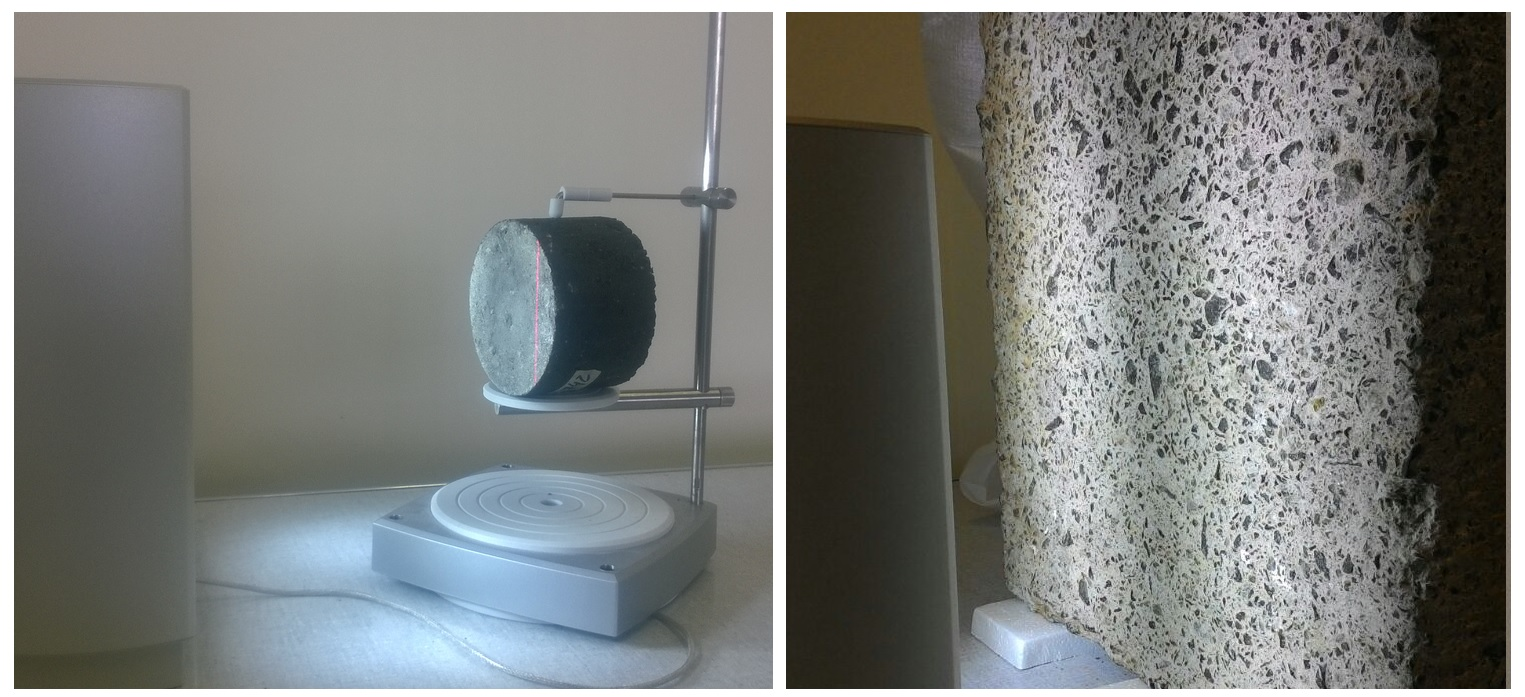
\includegraphics[scale=0.35]{figures/cps.jpg}}\\
\caption{Escaneamento de corpo de prova de asfalto cilíndrico e de placa de concreto.} 
\label{Fig:amostras}
\end{figure}

\subsection{Equipamento de escaneamento tridimensional a laser}
Neste estudo, foi utilizado o Next Engine\textsuperscript{\textregistered} laser scanner, cujas especificações técnicas estão descritas na Figura \ref{Fig:scanner}, a seguir:

\begin{figure}[!ht]
\centering
{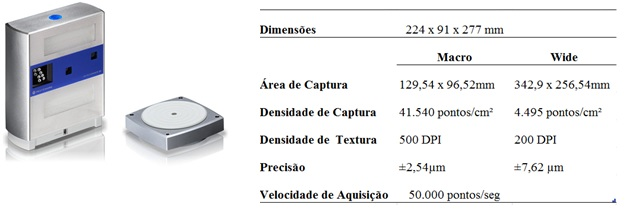
\includegraphics[scale=1]{figures/scanner.jpg}}\\
\caption{Equipamento de escaneamento tridimensional e especificações técnicas.}
\makebox[\width]{Fonte: Adaptado de \citeonline{nextengine}}\\
\label{Fig:scanner}
\end{figure}

De acordo com as especificações, não há definição de limite para o tamanho do objeto a ser escaneado. No caso de objetos cujas dimensões excederem o campo de alcance do equipamento pode ser feita uma captura em várias etapas por meio de um \emph{software} fornecido. 

O tempo de escaneamento de cada face é estimado em cerca de dois minutos, a partir da velocidade de aquisição dos dados que consta na tabela acima. 

Sobre as condições do ambiente, o equipamento pode ser utilizado em condições normais de iluminação, não sendo necessário nenhum requisito especial. 

O equipamento utiliza o MLT (\emph{Multistripe Laser Triangulation}) que é uma técnica estereoscópica\footnote{A estereoscopia é uma técnica antiga que utiliza imagens capturadas de um objeto em ângulos diferentes que permite através do uso de dispositivos de apreciação da imagem capturada a percepção das dimensões de altura largura e profundidade (3D) \cite{coutinho}.} baseada no Método da Interseção\footnote{O Método da Interseção também é conhecido como método das Coordenadas Bipolares. Este tipo de levantamento é usado em pequenas áreas que possuam um relevo um tanto quanto acidentado \cite{espartel}.}, a qual permite determinar a posição de um ponto no espaço a partir de um sistema de coordenadas referenciado.

Como descreve \citeonline{bitelli}, o equipamento emite um feixe de energia (laser) com um ângulo $\alpha$, previamente conhecido no processo de calibração; ao atingir a superfície do objeto localizado no Ponto A, sua posição é medida. A flexão do feixe de energia depende do tipo de material que compõe a superfície; parte do sinal refletido atinge o sensor (usualmente CCD ou CMOS) posicionado à uma distância conhecida, chamada de linha de referência (b), do emissor. O ângulo $\beta$ do raio refletido é desconhecido, porém pode ser inferido aplicando-se relações trigonométricas e tendo-se conhecimento da distância focal (c) e a posição do equipamento. Repetindo-se essa operação para vários pontos, podem ser determinadas suas coordenadas e a superfície em questão pode ser representada por meio de uma nuvem tridimensional de pontos.

\section{MÉTODOS}
O estudo foi conduzido de acordo com a metodologia esquematizada na Figura \ref{Fig:metodo}. As etapas podem ser classificadas em: ensaios experimentais, ensaios computacionais e análise dos resultados. A primeira consiste no Ensaio de Mancha de Areia e posterior extração dos corpos de prova (no caso dos pavimentos asfálticos), a segunda consiste no escaneamento dos corpos de prova em laboratório e processamento dos dados pelo algoritmo e por fim, a análise consiste na comparação dos dados obtidos em ambos os procedimentos e na determinação do erro relativo.  

\begin{figure}[!ht]
\centering
{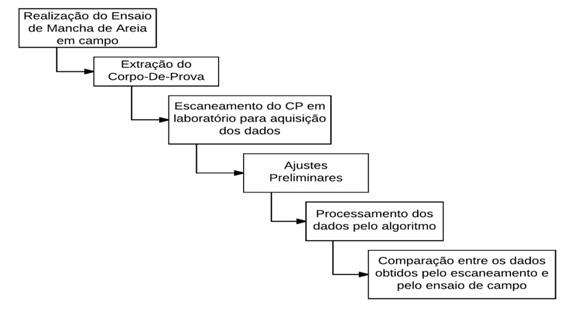
\includegraphics[scale=1]{figures/metodo.jpg}}\\
\caption{Descrição da metodologia utilizada} 
\label{Fig:metodo}
\end{figure}

\subsection{Método experimental: ensaio de Mancha de Areia}
Vários podem ser os parâmetros adotados para a análise da rugosidade dos pavimentos; optou-se pela utilização da  “textura superficial”, sendo esta medida intuitiva e amplamente utilizada pelo DNIT.

Um dos métodos de medição da textura de pavimentos é o ensaio da Mancha de Areia, que determina mais especificamente a macrotextura da superfície. Este ensaio é válido para pavimentos betuminosos e pavimentos rígidos de concreto cuja profundidade de textura seja maior que 0,25mm e é diretamente afetado pela constituição da mistura (distribuição de vazios, forma, tortuosidade) conforme afirma o estudo de \citeonline{pratico}.

O Ensaio de Mancha de Areia é normatizado pela ASTM E965:2006 \nocite{astme965} e foi realizado conforme suas especificações. A seguir, descreve-se o procedimento para sua realização: 
\begin{enumerate}
\item Deve ser escolhido um local protegido pelo vento, sendo possível instalar telas para formarem uma barreira de proteção, se necessário; 

\item Realiza-se a limpeza da superfície com o auxílio de uma escova ou pincel, removendo todos os resíduos que possam estar preenchendo os vazios; 

\item Enche-se o reservatório de areia, nivelando a areia com a borda do reservatório com auxílio de uma régua;

\item Verte-se o volume de areia na superfície do pavimento a ser avaliado;

\item Espalha-se o volume conhecido de material sobre a superfície com auxílio de um aparato emborrachado. Essa etapa deve ser feita com movimentos circulares de forma a criar uma forma mais próxima de um círculo possível; 

\item Efetua-se por meio de régua ou trena, quatro medições do diâmetro da mancha, tomando-se a média aritmética como o valor a ser adotado;

\item Calcula-se a profundidade Média da Macrotextura do Pavimento (MDT) por meio da Equação \ref{Eq:mdt}:
\begin{equation}\label{Eq:mdt}
%
MDT = \frac{4V}{\pi D^2}
%
\end{equation}
%
\end{enumerate}

Onde $V$ é volume de areia utilizado no ensaio e $D$ é média dos diâmetros obtidos através do círculo formado pela areia.

O parâmetro obtido pelo ensaio de Mancha de Areia é o MTD (\emph{Mean Texture Depth}) ou HS (\emph{Height of Sand}), o qual representa a rugosidade por meio da altura média de areia que preenche os vazios de um pavimento. Esse parâmetro obtido pode ser associado à textura do pavimento de acordo com a Tabela \ref{tab:alturadeareia}, a seguir: 
\vspace{0.5cm}
\begin{table}[htb!]
\centering
\caption{Comparação entre Altura de Areia e a Textura do Pavimento}
\label{tab:alturadeareia}
\begin{tabular}{cc}
\hline
Altura de Areia HS & \multicolumn{1}{c}{Textura Superficial} \\ \hline
HS < 0,20mm              & Muito fina ou Muito fechada                            \\
0,20mm < HS < 0,40mm              & Fina ou fechada                            \\
0,40mm < HS < 0,80mm              & Média                           \\
0,80mm < HS < 1,20mm              & Grosseira ou Aberta                         \\
HS > 1,20mm              & Muito grosseira ou Muito aberta                            \\ \hline
\vspace{0cm}
\end{tabular}\\
\makebox[\width]{Fonte: DER-MG (2005)
\nocite{dermg}}\\
\end{table}

Como citado anteriormente, a textura exerce grande influência nas características da superfície do pavimento. A resistência à derrapagem é uma destas características, que está associada à segurança dos usuários. A relação entre os valores de MTD e as classes de resistência à derrapagem está descrita na Tabela \ref{tab:resistencia}, também estão descritas as correlações com o Coeficiente de Atrito Longitudinal (CAL) e Valor de Resistência à Derrapagem (VRD). 
\vspace{0.5cm}
\begin{table}[htb!]
\centering
\caption{Relação entre a resistência à derrapagem, macrotextura e coeficiente de atrito}
\label{tab:resistencia}
\begin{tabular}{cccc}
\hline
\pbox{20cm}{Classes de Resistência \\ { }{ } \centering à Derrapagem} & \pbox{20cm}{Macrotextura \\ do pavimento} & \pbox{20cm}{CAL}& \pbox{20cm}{VRD} \\ \hline
Perigosa  & -  &<0,24  &<25		                           \\
Muito Lisa  & Muito Fina ou Muito fechada  &0,24-0,30  &25-31                            
\\
Lisa  &Fechada  &0,31-0,37  &32-39
\\
Pouco Rugosa  &Fechada  &0,38-0,44  &40-46                 \\
Medianamente Rugosa  &Média  &0,45-0,51  &47-64
\\
Rugosa  &Grosseira ou Aberta  &0,52-0,72  &65-75 
\\
Muito Rugosa  &Muito Grosseira ou Muito Aberta  &>0,72  &>75 \\ \hline
\vspace{0cm}
\end{tabular}\\
\makebox[\width]{Fonte: DER-MG (2005)}
\end{table}

Segundo a especificação da norma DNIT 031:2006 \nocite{dnit031}, para atender às condições de segurança, o revestimento de concreto asfáltico acabado deve apresentar uma Altura de Areia dentro do intervalo 1,20mm $\geq$ HS $\geq$ 0,60mm. Ou seja, sua textura deve ter classificação média ou grosseira. Valores acima ou abaixo dos limites estabelecidos indicam que  o pavimento não está em condições adequadas ao uso. 

O método volumétrico da Mancha de Areia mostrou-se adequado às necessidades desta pesquisa por ser um ensaio de fácil execução e requerer aparatos simples. Além disso, justifica-se sua aplicação, uma vez que o parâmetro de textura obtido (MTD) pode ser facilmente correlacionado com os resultados computacionais. 

Contudo, como descrito por \citeonline{kuchiishi}, este procedimento está sujeito a erros, provenientes por exemplo da imprecisão do operador que manipula o disco espalhador e efetua as medidas necessárias. Além disso, ele não fornece uma análise completa da superfície do pavimento, pois a partir do valor médio de MTD não é possível inferir se a textura é positiva ou negativa, limitação que não ocorre no processo computacional.

Para minimizar os erros de operação, este ensaio foi realizado sucessivamente cinco vezes em cada pavimento analisado, antes da extração do corpo de prova nessa região. Adotou-se o MTD do pavimento como a média aritméticas das medidas, sendo excluídas aquelas cujo desvio tenha sido $\pm10\%$ em relação à média. 

\subsection{Método computacional: escaneamento tridimensional}
A tecnologia de escaneamento tridimensional permite a representação de objetos de grande complexidade, o resultado do escaneamento é uma nuvem de pontos 3D que representa com precisão o objeto escaneado. O processamento da nuvem de pontos permite a determinação automática de parâmetros de difícil medição manual como a textura.

Os erros que ocorrem no processo de escaneamento a laser são ocasionados por desvios das condições ideais. Há uma variedade de aspectos que podem influenciar negativamente o desempenho dos equipamentos, reduzindo sua precisão ou até mesmo culminando em falha na medição. Alguns destes aspectos principais são: iluminação insuficiente do ambiente, formato e cor do objeto, trepidações da superfície em que se encontra o equipamento. Os problemas derivados destas falhas costumam estar relacionados ao desvio da posição geométrica da nuvem de pontos em relação à sua posição real, o que gera um modelo impreciso. Por essa razão, durante a fase de aquisição dos dados todas as precauções devem ser tomadas a fim de que se obtenha a representação mais exata possível.

Para a análise computacional dos dados obtidos através do escaneamento tridimensional a laser foi realizado o procedimento computacional de forma que toda a superfície fosse utilizada para aproximação da rugosidade. O método consiste nas seguintes etapas:
\begin{enumerate}
\item Leitura do conjunto de dados e o processamento para a retirada da superfície de interesse. O tratamento dos dados provenientes do scanner foi necessário pela presença de valores atípicos e partes que não pertencem ao objeto influenciarem de forma negativa no cálculo dos parâmetros de rugosidade. Para isso, o algoritmo filtra e retira os pontos que estiverem fora de uma distância radial estabelecida;

\item Orientação correta dos dados. Em alguns casos o conjunto de pontos pode apresentar um ângulo em relação ao plano x-y, o que impossibilita a análise efetiva da rugosidade. Com o objetivo de orientar os pontos na direção de maior variação, foi utilizada a técnica Análise de Componentes Principais (PCA)\footnote{A Análise de Componentes Principais é uma técnica da estatística que
consiste em transformar um conjunto de variáveis originais em outro conjunto de variáveis
de mesma dimensão denominadas de componentes principais \cite{varella}.} de forma que a direção de maior variação fique orientada no eixo-x e a de menor variação no eixo-z que será utilizado para o cálculo da profundidade;

\item Separação da superfície por meio de planos transversais para que todos os dados capturados pelo scanner fossem utilizados. O centroide da superfície é determinado através das médias das distâncias dos eixos coordenados, sendo utilizado como referência para a divisão dos planos radiais;

\item Determinação dos pontos pertencentes a cada seção. A superfície foi cortada por 19 planos radiais rotacionados em torno do centroide separados por 9$^{\circ}$ entre si. Para cada ponto $p = (px, py, pz)$ da nuvem de pontos é verificada a distância d do plano ao ponto de forma o ponto pertence à seção se $|d|<\Delta y$. Na Figura \ref{Fig:perfil} podemos ver a representação em duas dimenções de uma das seções utilizadas pelo algoritmo;

\item Cálculo do volume da seção. O algoritmo determina o volume abaixo da superfície para cada seção definida anteriormente e interpreta como aproximação do volume de um prisma de base retangular. Dessa forma, a altura possa ser encontrada diretamente através da Equação \ref{Eq:prisma} do volume deste prisma.
\begin{equation}
\label{Eq:prisma}
h = \frac{V}{A B}
\end{equation}

\noindent Onde $h, V, A$ e $B$ se referem a altura do prisma, volume, comprimento e profundidade respectivamente.

\item Posteriormente o algoritmo calcula a média das alturas obtidas para cada seção e retorna o valor aproximado para a profundidade média do perfil (MPD).

\begin{figure}[!ht]
\centering
{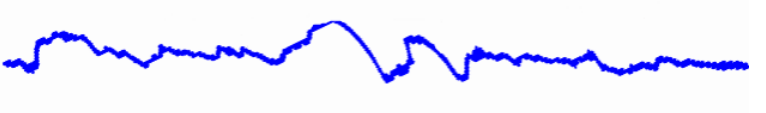
\includegraphics[scale=0.7]{figures/perfil.jpg}}\\
\caption{Seção transversal obtida pelo algoritmo.} 
\makebox[\width]{Os pontos foram projetados no plano-xz para visualização em 2 dimensões.} 
\label{Fig:perfil}
\end{figure}
\end{enumerate}

Para o caso do pavimento rígido, em que foi utilizada uma placa de concreto, foi necessário uma etapa extra que consistiu na extração de uma região circular a partir da área total escaneada (Figura \ref{Fig:placaecp}). Este procedimento foi necessário para que as áreas analisadas fossem similares para ambos os pavimentos. 

\begin{figure}[!ht]
\centering
{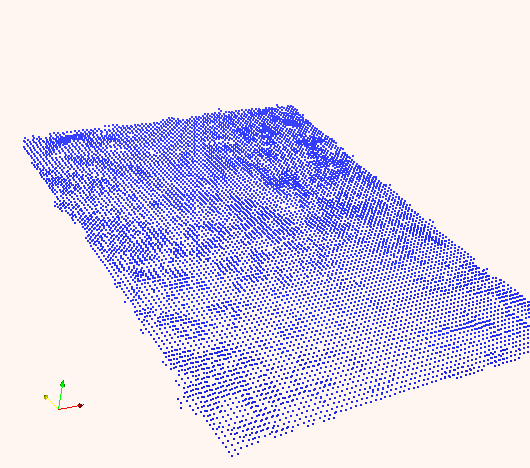
\includegraphics[scale=0.5]{figures/placa.jpg}}\\
\caption{Área escaneada para o pavimento rígido.}
\label{Fig:placaecp}
\end{figure}

\begin{figure}[!ht]
\centering
{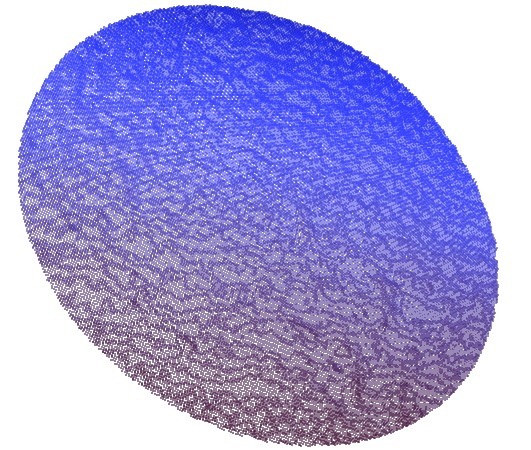
\includegraphics[scale=0.5]{figures/cp2.jpg}}\\
\caption{Delimitação da área para análise.}
\label{Fig:placaecp}
\end{figure}

Foram realizados testes com a aquisição de 3 e de 6 leituras por corpo de prova. A cada leitura a amostra foi rotacionada, para que nenhuma área ficasse encoberta e todos os pontos fossem escaneados. O \emph{software ScanStudio}, fornecido pelo próprio fabricante realizou a sobreposição destas, por meio de pontos referência nas superfícies dos corpos de prova, gerando um modelo final único para cada uma das quatro amostras.

O escanamento foi realizado nos modos “\emph{Macro}” e “\emph{Wide}” e o equipamento foi ajustado para a melhor qualidade. Nestes parâmetros, cada escanemanto levou em torno de 180 segundos. Ao final do processo de escaneamento da amostra obtêm-se um arquivo no formato \emph{*.xyz}. 

O arquivo obtido foi processado por um algoritmo desenvolvido na linguagem \emph{Phyton}, o mesmo utlizado por \citeonline{simmec}. Além de retornar a rugosidade média e o erro percentual em relação aos dados experimentais, o algoritmo também calcula alguns parâmetros estatísticos como desvio padrão, mediana e curtose, definidos na seção 2.2, que foram utilizados para verificar a precisão dos resultados.   

 

